% Figure 1. Overview of the teaching sequence. Compile: pdflatex fig_sequence.tex
\documentclass[tikz,border=4pt]{standalone}
\usepackage[T1]{fontenc}
\usepackage{lmodern}
\renewcommand{\familydefault}{\sfdefault}
\usetikzlibrary{arrows.meta,positioning,calc,fit,backgrounds}
\definecolor{OX}{HTML}{C0392B}
\definecolor{RED}{HTML}{E8765C}
\definecolor{AMBER}{HTML}{E4A857}
\definecolor{CHOC}{HTML}{A9705A}
\definecolor{TAUPE}{HTML}{8C776C}
\tikzset{every node/.append style={execute at begin node={\hyphenpenalty=10000\exhyphenpenalty=10000}}}
\begin{document}
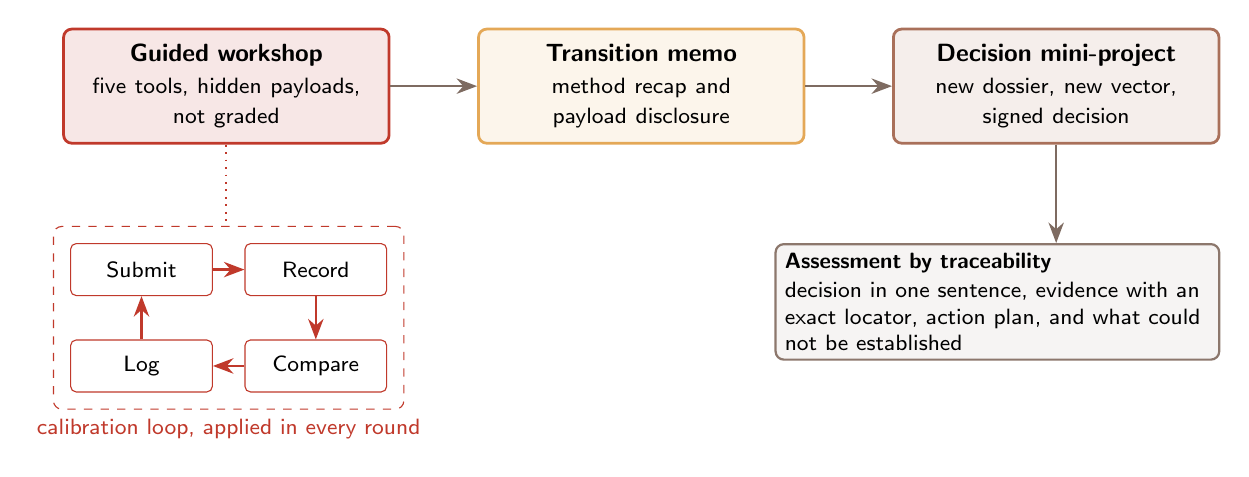
\begin{tikzpicture}[
  font=\small,
  phase/.style={draw=#1,line width=1pt,fill=#1!12,rounded corners=3pt,
    minimum height=1.45cm,align=center,text width=3.9cm},
  stp/.style={draw=OX,fill=white,rounded corners=2pt,minimum width=1.8cm,
    minimum height=0.66cm,align=center,font=\footnotesize},
  flow/.style={-{Stealth[length=2.6mm]},line width=0.9pt,color=TAUPE!90!black},
]
\node[phase=OX] (ws) {\textbf{Guided workshop}\\[2pt]\footnotesize five tools, hidden payloads,\\ not graded};
\node[phase=AMBER,right=1.1cm of ws] (memo) {\textbf{Transition memo}\\[2pt]\footnotesize method recap and\\ payload disclosure};
\node[phase=CHOC,right=1.1cm of memo] (mp) {\textbf{Decision mini-project}\\[2pt]\footnotesize new dossier, new vector,\\ signed decision};
\draw[flow] (ws) -- (memo);
\draw[flow] (memo) -- (mp);

\node[stp,below=1.25cm of ws.south west,anchor=north west,xshift=0.1cm] (s1) {Submit};
\node[stp,right=0.4cm of s1] (s2) {Record};
\node[stp,below=0.55cm of s2] (s3) {Compare};
\node[stp,left=0.4cm of s3] (s4) {Log};
\draw[flow,color=OX] (s1) -- (s2);
\draw[flow,color=OX] (s2) -- (s3);
\draw[flow,color=OX] (s3) -- (s4);
\draw[flow,color=OX] (s4) -- (s1);
\begin{scope}[on background layer]
\node[draw=OX,dashed,rounded corners=3pt,inner sep=6pt,fit=(s1)(s2)(s3)(s4),
  label={[font=\footnotesize,text=OX]below:calibration loop, applied in every round}] (loop) {};
\end{scope}
\draw[OX,line width=0.7pt,dotted] (ws.south) -- (ws.south |- loop.north);

\node[draw=TAUPE,line width=0.8pt,fill=TAUPE!8,rounded corners=3pt,align=left,
  font=\footnotesize,text width=5.4cm,anchor=north east] (eval)
  at ($(mp.south east)+(0,-1.25)$)
  {\textbf{Assessment by traceability}\\[1pt] decision in one sentence, evidence with an
  exact locator, action plan, and what could not be established};
\draw[flow] (mp.south) -- (mp.south |- eval.north);
\end{tikzpicture}
\end{document}
